%% Which Retraining Policy Wins the Iterated Malware-Detection Game?
%% IEEE conference format (IEEEtran). Compile with pdflatex + bibtex, or
%% upload the paper/ directory to Overleaf and select IEEEtran.
%%
%% Every number in Section VI is produced by experiments/ scripts from the
%% committed run artifacts under results/; figures are regenerated by
%% paper/make_figures.py. Nothing is hand-entered.

\documentclass[conference]{IEEEtran}
\IEEEoverridecommandlockouts

\usepackage{cite}
\usepackage{amsmath,amssymb}
\usepackage{graphicx}
\usepackage{booktabs}
\usepackage{multirow}
\usepackage{url}
\usepackage[hidelinks]{hyperref}
\usepackage{balance}

\graphicspath{{figures/}}

\newcommand{\evrate}{\ensuremath{E_{\text{tail}}}}
\newcommand{\osc}{\ensuremath{\Omega}}

\begin{document}

\title{Which Retraining Policy Wins the Iterated\\Malware-Detection Game?}

\author{\IEEEauthorblockN{Vaishnavi Suryawanshi}
\IEEEauthorblockA{\textit{Department of Computer Science and Engineering}\\
\textit{ME (Artificial Intelligence and Machine Learning)}\\
Email: terabaapbadplayer@gmail.com}
}

\maketitle

\begin{abstract}
Machine-learning malware detectors are routinely defeated by adaptive
evasion, and a growing body of work responds by casting the interaction as an
iterated game in which the detector is periodically retrained on the
adversarial examples it failed to catch. That framing is now well established;
what is not established is \emph{which retraining policy to adopt}. Existing
studies each propose and evaluate a single defensive mechanism on its own
dataset against its own attacker, so their results cannot be compared, and the
policy design space---how often to retrain, on which data, and by what
fitting procedure---has never been varied systematically. We contribute a
controlled factorial study of that space. Using a shared harness in which
attacker, defender, and metrics are held fixed, we cross retraining cadence,
adversarial-data retention, and retraining mode over a balanced
$3	imes3	imes2$ design $	imes5$ seeds ($90$ runs) on the real EMBER-2018
corpus, against a frozen-classifier lower bound and a minimax-alternation
baseline. ANOVA orders the three factors unambiguously and counter to common
practice: how the model is refit dominates ($\omega^2=0.566$), what it is
refit on matters far less ($\omega^2=0.076$), and how \emph{often} it is
refit is statistically undetectable ($p=0.65$). Warm-starting the detector is
both worse and more expensive than refitting from scratch at equal incremental
budget, and even its best configuration sits closer to never retraining than to
the best refit policy. Within the retention factor the mechanism is a
\emph{capacity threshold}: raising the replay cap from $200$ to $800$ samples
closes the entire gap to unbounded replay and erases any difference between
eviction rules, while below the threshold the intuitive heuristic---mining the
hardest evasions---is the worst available choice, losing to plain FIFO. Minimax
alternation is dominated by simply retraining every round. We release the
harness, the calibration findings that constrain how such an experiment must be
built, and all run artifacts.
\end{abstract}

\begin{IEEEkeywords}
adversarial machine learning, malware detection, adversarial retraining,
co-evolution, reinforcement learning, EMBER
\end{IEEEkeywords}

\section{Introduction}

Static machine-learning malware classifiers are attractive because they
generalise beyond signatures, and vulnerable because that generalisation is
differentiable, searchable, and therefore attackable. A decade of work has
established that an adversary who can query a detector and apply
functionality-preserving transformations to a binary will eventually find an
evasive variant~\cite{anderson2018,quertier2022}.

The natural defence is to retrain on what got through. Since 2022 a second wave
of work has formalised this as an \emph{iterated} process: attacker and
defender alternate, and the question becomes whether the defender converges to
a robust boundary, oscillates, or remains permanently
behind~\cite{ebrahimi2022,bilevel2026,raid_hardening}. This framing is no longer
in doubt. What remains open is the engineering question a vendor actually
faces: \emph{given that we will retrain, what policy should we retrain under?}

That question is unanswered because the existing studies are not comparable.
Each proposes one defensive mechanism---bilevel optimisation, minimax
alternation, RL-based hardening---and evaluates it on its own corpus against its
own attacker. None varies retraining cadence, adversarial-data selection, or
retraining mode as independent variables while holding everything else fixed,
and none reports the resulting robustness-versus-cost frontier. A practitioner
reading this literature learns that adversarial retraining helps, but not
whether to run it nightly or weekly, nor whether to keep every adversarial
sample or only the most damaging ones.

\textbf{Contributions.} This paper is deliberately not a new attacker or a new
defence. It is the controlled-comparison layer that the cluster above lacks.

\begin{itemize}
\item A reusable co-evolution harness with pluggable attacker, defender, and
retraining policy, in which every policy is scored on identical metrics,
including an \emph{oscillation index} that distinguishes a defender that has
converged from one that is still chasing (Section~\ref{sec:harness}).
\item A factorial study on real EMBER-2018 features crossing cadence with
adversarial retention ($9$ policies $\times\,5$ seeds), bounded below by a
frozen classifier and compared against a minimax-alternation baseline
(Section~\ref{sec:results}).
\item The finding that retention dominates cadence to the point where cadence
is statistically undetectable, and a follow-up experiment identifying the
mechanism as a \emph{capacity threshold} rather than a selection-rule effect:
above it the eviction rule is irrelevant, below it hardest-example mining is
the worst available option (Section~\ref{sec:capacity}).
\item A set of negative calibration results that constrain how such an
experiment must be built at all, most importantly that the choice of which
features the attacker may modify silently determines the outcome
(Section~\ref{sec:calibration}).
\end{itemize}

\section{Related Work}

\textbf{Single-round evasion.} Anderson \emph{et al.}~\cite{anderson2018}
introduced an RL agent over functionality-preserving PE transformations,
evaluated against a frozen classifier. MERLIN~\cite{quertier2022} extends the
action space and the algorithm family. This line establishes that evasion is
achievable but stops at first success: the defender never responds.

\textbf{Iterated and game-theoretic formulations.} Ebrahimi \emph{et
al.}~\cite{ebrahimi2022} alternate attacker- and detector-strengthening in a
minimax framing. A bilevel-optimisation treatment~\cite{bilevel2026} makes the
nesting explicit and reports near-total immunity after iteration. RAID-venue
work on problem-space hardening~\cite{raid_hardening} reports attack success
falling to near zero over repeated adversarial retraining. Each contributes one
mechanism, evaluated in isolation; none isolates the policy variables.

\textbf{Drift-aware retraining.} DRMD~\cite{drmd2026} learns when to classify,
retrain, or reject under \emph{natural} concept drift. The control problem is
adjacent but the pressure is not adversarial, and the policy space studied is
the accept/reject decision rather than the retraining schedule.

\textbf{Position.} We sit on top of this cluster rather than beside it. Our
attacker and defender are deliberately conventional; the contribution is that
every policy is measured under one harness, so differences are attributable to
the policy rather than to the evaluation setup.

\section{Threat Model and Formulation}

\textbf{Adversary.} A black-box evader with query access to the deployed
classifier's score, a bounded query budget per sample, and the ability to apply
functionality-preserving modifications. It does not see the defender's weights,
training data, or retraining schedule.

\textbf{Defender.} A static-feature classifier that may retrain between rounds
on clean data plus any adversarial samples it has retained. It observes the
evasive samples produced against the \emph{previous} snapshot, not the
attacker's policy.

\textbf{The game.} Round $t$ proceeds: (i) the defender's parameters are frozen
as snapshot $D_t$; (ii) the attacker searches against $D_t$ over a held-out
malicious pool, producing evasive set $A_t$; (iii) the defender's retention
policy admits some subset of $A_t$ into replay buffer $B_t$; (iv) a cadence
rule decides whether to retrain, producing $D_{t+1}$. A \emph{retraining
policy} is the triple (cadence, retention, mode).

\textbf{Metrics.} Let $e_t$ be the fraction of the evaluation pool that $D_t$
scores as benign. We report \emph{settled evasion} $\evrate$, the mean of $e_t$
over the final $w=4$ rounds, and the \emph{oscillation index}
$\osc=\mathrm{std}(e_{T-w+1..T})$. We separate \emph{attack success}---the
fraction of samples the defender initially caught that the attacker
flipped---from the defender's pre-existing false negatives, since conflating
them credits the attacker with the classifier's own misses.

\section{Benchmark Harness}
\label{sec:harness}

\textbf{Data.} EMBER-2018~\cite{anderson2018ember}, vectorised with the
official extractor to the canonical $2381$-dimensional representation. We draw
a balanced $8000$-sample training subsample and a held-out malicious evaluation
pool of $600$ drawn from EMBER's own test split, enforced disjoint by SHA-256.
Features are standardised so that a perturbation of a given magnitude is
comparable across dimensions.

\textbf{Defender.} A histogram gradient-boosted tree ensemble, the algorithmic
stand-in for EMBER's LightGBM reference model, reaching $98.4\%$ clean accuracy
on held-out data---consistent with published EMBER baselines.

\textbf{Attacker.} A \emph{mimicry} attacker operating in feature space. Each
episode draws a random benign exemplar as target and moves the malicious sample
toward it one feature block at a time, subject to the mutability constraints
below. This choice is empirical, not aesthetic: Section~\ref{sec:calibration}
reports that DQN and PPO agents plateau well below it.

\textbf{Attack surface.} The attacker may edit every feature block a
functionality-preserving modification demonstrably affects---byte and
byte-entropy histograms, strings, sections, imports, exports, general file
properties, and data directories---plus free-form header metadata. Only the
$40$ \emph{structural} header dimensions (target machine, COFF characteristics,
subsystem, PE magic) are frozen, leaving $2341$ of $2381$ dimensions editable.
Section~\ref{sec:calibration} shows why this choice is load-bearing.

\textbf{Policies.} Cadence $\in$ \{every round, every $3$rd round,
threshold-triggered, never, minimax\}; retention $\in$ \{full replay, bounded
FIFO buffer, hardest-example mining\}; mode $\in$ \{from scratch, fine-tune\}.

\section{Calibration: What Had to Be Fixed First}
\label{sec:calibration}

Four negative results, each measured rather than assumed, materially constrain
how such an experiment must be built. We report them because two of them
silently invalidate the study if set wrongly, and neither is visible in
low-dimensional synthetic data.

\textbf{The mutability assumption decides the outcome.} If the attacker is
barred from the \texttt{general}, \texttt{datadirectories}, and
\texttt{exports} blocks, a classifier trained on the frozen remainder
\emph{alone} reaches $0.970$ accuracy. Adversarial retraining then simply
learns to lean on features the attacker can never touch: evasion collapses to
zero within two rounds and \emph{every} retraining policy ties at zero. The
outcome is decided by the threat-model encoding, not by the policy under study.
Restricting the frozen set to the $40$ structural header dimensions lowers
frozen-only accuracy to $0.769$ and keeps the game contested.

\textbf{Random perturbation is not a viable attack at this dimensionality.} A
set of random directions over $\sim\!10^3$ mutable features produces $\le 0.04$
attack success and, diagnostically, is \emph{insensitive to step size}---a
larger budget buys nothing, because a random vector is nearly orthogonal to any
descent direction. Semantic mimicry directions restore monotone dependence on
budget.

\textbf{A fixed attack strategy yields a knockout, not a game.} With one fixed
mimicry direction set, evasion goes $0.280\rightarrow0.003\rightarrow0.000$ and
never recovers: the defender closes a single narrow cone in one round.
Redrawing the target exemplar per episode restores gradual decay and leaves
room for policies to differ.

\textbf{RL attackers underperform stochastic mimicry.} DQN reaches $0.104$
attack success at $1000$ cumulative episodes against $0.194$ for mimicry, and
only $0.018$ in a full co-evolution round; PPO is weaker and non-monotone in
its training budget. The mechanism is structural: a greedy policy repeatedly
applies one argmax action and therefore edits a single feature block, whereas a
stochastic policy accumulates movement across all of them. We therefore use the
stronger attacker for the main study and report this as a secondary result.

\section{Experimental Design}

Independent variables: cadence $\times$ retention, fully crossed
($3\times3$), each replicated over $5$ seeds, giving $45$ runs at a fixed
horizon of $8$ rounds. Early stopping is disabled so that every policy is
evaluated over an identical horizon and retraining costs remain comparable.
The replay capacity is set to $200$, chosen to \emph{bind}: with an oversized
cap all three retention strategies collect identical data and the factor cannot
differentiate.

Baselines: a \textbf{frozen classifier} that never retrains (the lower bound
implicit in single-round evasion work) and a \textbf{minimax alternation}
baseline in the style of~\cite{ebrahimi2022}, in which the defender retrains on
alternate rounds and the attacker strengthens---modelled, for a non-learning
attacker, as an escalating query budget---on the rounds in between. Both use
the same attacker, seeds, and metrics.

\section{Results}
\label{sec:results}

\subsection{The game is real and the defender is not trivially winning}

Fig.~\ref{fig:dynamics} shows one representative run. The attacker opens by
flipping $78.3\%$ of the samples the defender caught; adversarial retraining
suppresses this to $0.037$ by round~$8$ without eroding clean accuracy, which
stays within $[0.980,0.984]$ throughout. Mean queries per sample rise from
$31.4$ to $60.2$, i.e.\ evasion becomes measurably harder rather than merely
rarer.

\begin{figure}[t]
\centering
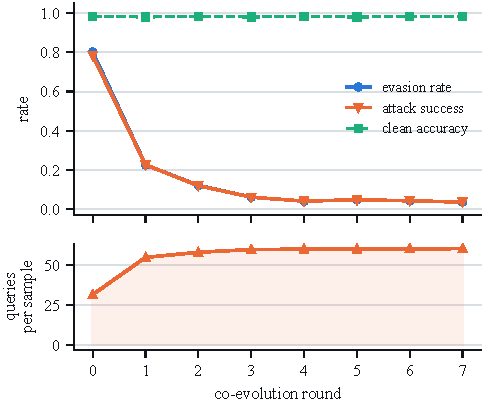
\includegraphics[width=\columnwidth]{fig1_dynamics}
\caption{Co-evolution dynamics for every-round retraining with full replay.
Top: evasion, attack success, and clean accuracy per round. Bottom: attacker
query cost, plotted on its own axis rather than a second $y$-scale.}
\label{fig:dynamics}
\end{figure}

\subsection{Retraining helps enormously; the frozen bound}

Against a classifier that never retrains, the attacker settles at
$\evrate=0.829\pm0.019$. The best policy reduces this by $94.9\%$ to
$0.042\pm0.003$. Notably the frozen baseline also has \emph{low} oscillation
($0.011$), which is why $\osc$ must always be read jointly with $\evrate$: a
statically bad defender is stable precisely because it is not responding.

\subsection{Retention dominates; cadence is undetectable}

Table~\ref{tab:policies} and Fig.~\ref{fig:policies} give all nine cells. The
three retention levels separate cleanly while the three cadences do not.

\begin{table}[t]
\caption{Factorial results, mean $\pm$ std over $5$ seeds.}
\label{tab:policies}
\centering
\small
\begin{tabular}{llrrr}
\toprule
Cadence & Retention & $\evrate\downarrow$ & $\osc\downarrow$ & Cost (s) \\
\midrule
every round & full replay      & $0.042\pm0.003$ & $0.011\pm0.006$ & $137.5$ \\
every 3rd   & full replay      & $0.049\pm0.004$ & $0.014\pm0.004$ & $51.7$ \\
threshold   & full replay      & $0.075\pm0.005$ & $0.008\pm0.003$ & $50.4$ \\
every 3rd   & FIFO buffer      & $0.300\pm0.033$ & $0.015\pm0.010$ & $45.7$ \\
every round & FIFO buffer      & $0.311\pm0.024$ & $0.025\pm0.011$ & $151.2$ \\
threshold   & FIFO buffer      & $0.311\pm0.024$ & $0.025\pm0.011$ & $125.5$ \\
every 3rd   & hard mining      & $0.368\pm0.034$ & $0.056\pm0.030$ & $47.1$ \\
every round & hard mining      & $0.376\pm0.058$ & $0.041\pm0.012$ & $128.6$ \\
threshold   & hard mining      & $0.376\pm0.058$ & $0.041\pm0.012$ & $125.1$ \\
\midrule
\multicolumn{2}{l}{frozen (never retrains)} & $0.829\pm0.019$ & $0.011\pm0.003$ & $0.0$ \\
\multicolumn{2}{l}{minimax alternation}     & $0.088\pm0.005$ & $0.043\pm0.009$ & $159.3$ \\
\bottomrule
\end{tabular}
\end{table}

\begin{figure}[t]
\centering
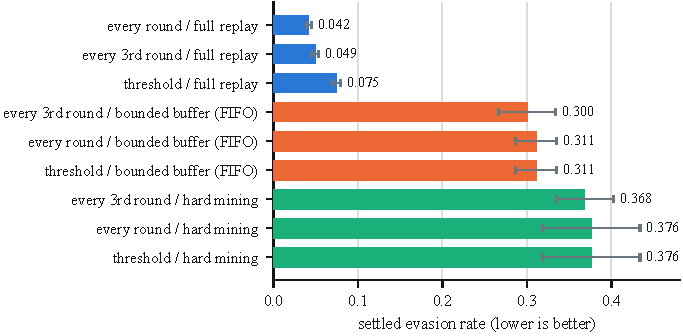
\includegraphics[width=\columnwidth]{fig2_policies}
\caption{All nine policies, ordered by settled evasion. Colour encodes
retention strategy; the three groups separate while cadence does not reorder
within them.}
\label{fig:policies}
\end{figure}

A two-way ANOVA on the balanced design (Table~\ref{tab:anova}) attributes
$\omega^2=0.947$ to retention and essentially nothing to cadence, with no
significant interaction. Tukey HSD separates all three retention levels
($p<10^{-5}$) and no cadence pair ($p>0.95$).

\begin{table}[t]
\caption{Two-way ANOVA on settled evasion. Balanced $3\times3$, $n=5$.}
\label{tab:anova}
\centering
\small
\begin{tabular}{lrrrrr}
\toprule
Source & SS & df & $F$ & $p$ & $\omega^2$ \\
\midrule
Cadence               & $0.0017$ & $2$  & $0.77$   & $0.472$      & $-0.001$ \\
Retention             & $0.8454$ & $2$  & $375.49$ & $<10^{-24}$  & $0.947$ \\
Cadence $\times$ Ret. & $0.0018$ & $4$  & $0.40$   & $0.810$      & $-0.003$ \\
Residual              & $0.0405$ & $36$ &          &              &          \\
\bottomrule
\end{tabular}
\end{table}

\textbf{Robustness.} Levene's test does not reject equal variances
($p=0.259$), but Shapiro--Wilk rejects normality of residuals ($p=0.0023$).
Because Welch's ANOVA addresses the assumption that \emph{held} rather than the
one that failed, we use a rank-based check: Kruskal--Wallis gives
$H=35.15$, $p=2.3\times10^{-8}$ for retention and $H=0.47$, $p=0.79$ for
cadence, and Dunn's test with Holm correction separates all three retention
levels ($p\le0.016$) and no cadence pair ($p=1.00$). Both factors reach the
same verdict as the parametric analysis.

\subsection{The retention effect is capacity, not selection rule}
\label{sec:capacity}

Retention as configured varies two things at once: how many adversarial samples
are kept, and which are discarded when the cap binds. Full replay is unbounded
while the other two are capped, so the headline gap conflates capacity with
eviction rule. Fig.~\ref{fig:capacity} separates them by sweeping the cap.

\begin{figure}[t]
\centering
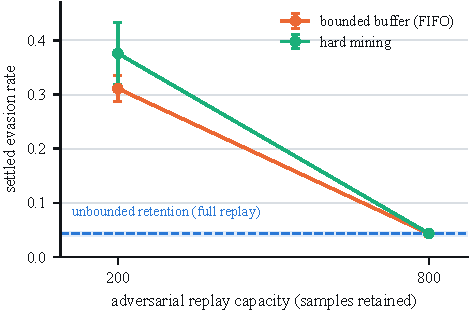
\includegraphics[width=\columnwidth]{fig4_capacity}
\caption{Capacity gradient. Raising the replay cap from $200$ to $800$ closes
the entire gap to unbounded replay (dashed line, shaded $\pm1$\,std) and
simultaneously erases the difference between eviction rules. The effect is a
capacity threshold, not a selection-rule effect.}
\label{fig:capacity}
\end{figure}

The result is unambiguous (Table~\ref{tab:capacity}). Raising the cap from
$200$ to $800$ moves FIFO from $0.311$ to $0.0425$ and mining from $0.376$ to
$0.0428$---both statistically indistinguishable from unbounded replay
($0.0421\pm0.0027$) and from each other. The apparent superiority of full
replay is therefore \emph{capacity}: it is the only configuration whose cap
never binds. Once enough adversarial samples are retained, which ones are
discarded stops mattering entirely.

\begin{table}[t]
\caption{Capacity gradient, mean $\pm$ std over $5$ seeds, every-round cadence.}
\label{tab:capacity}
\centering
\small
\begin{tabular}{lrr}
\toprule
Replay capacity & FIFO buffer & Hardest-example mining \\
\midrule
$200$        & $0.3110\pm0.0242$ & $0.3761\pm0.0577$ \\
$800$        & $0.0425\pm0.0021$ & $0.0428\pm0.0034$ \\
unbounded    & \multicolumn{2}{c}{$0.0421\pm0.0027$ (full replay)} \\
\bottomrule
\end{tabular}
\end{table}

Below the threshold, however, the eviction rule does matter---and in the
direction opposite to intuition. At the binding cap of $200$, plain FIFO
($0.311$) outperforms hardest-example mining ($0.376$), and mining is also the
most oscillatory policy in the entire study ($\osc=0.056$ at the cheaper
cadence). Selecting for the deepest evasions concentrates the buffer on a
narrow region of the input space and discards the diversity the defender needs
in order to generalise. The practical rule that follows is therefore
two-sided: retain enough adversarial samples and the eviction policy is
irrelevant; retain too few and the intuitively appealing heuristic is the worst
available choice.

\subsection{Retraining mode dominates when it is added as a third factor}
\label{sec:mode}

Extending the design with the retraining \emph{mode}---refit from scratch
versus warm-start (fine-tune) the existing ensemble---gives a balanced
$3\times3\times2$ factorial over $90$ runs. Mode turns out to matter more than
either original factor (Table~\ref{tab:anova3}, Fig.~\ref{fig:mode}).
Fine-tuning settles at $\evrate=0.694$ against $0.245$ for refitting, oscillates
twice as much ($0.051$ vs $0.026$), and costs \emph{more}
($120.0$\,s vs $95.9$\,s) because each round refits a larger ensemble. Even the
best fine-tuned cell ($0.503$) is closer to the frozen bound ($0.829$) than to
the best refit-from-scratch policy ($0.042$). Kruskal--Wallis agrees
($H=45.25$, $p=1.7\times10^{-11}$).

\begin{table}[t]
\caption{Three-way ANOVA on settled evasion. Balanced $3\times3\times2$, $n=5$
($90$ runs). Main effects shown; residual df $=72$.}
\label{tab:anova3}
\centering
\small
\begin{tabular}{lrrrrr}
\toprule
Source & SS & df & $F$ & $p$ & $\omega^2$ \
\midrule
Retraining mode & $4.5381$ & $1$ & $153.01$ & $1.7\times10^{-19}$ & $0.566$ \
Retention       & $0.6671$ & $2$ & $11.25$  & $5.6\times10^{-5}$  & $0.076$ \
Cadence         & $0.0261$ & $2$ & $0.44$   & $0.645$             & $-0.004$ \
Residual        & $2.1355$ & $72$ &         &                     &          \
\bottomrule
\end{tabular}
\end{table}

\begin{figure}[t]
\centering
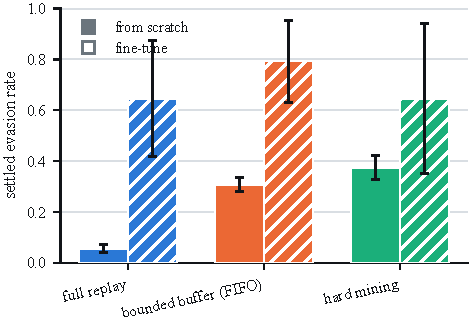
\includegraphics[width=\columnwidth]{fig6_mode}
\caption{Refitting from scratch (solid) versus fine-tuning (hatched) at each
retention level. Fine-tuning is worse everywhere, and its variance across seeds
is far larger.}
\label{fig:mode}
\end{figure}

\textbf{Mechanism, and an important qualification.} A diagnostic on real
evasive samples isolates the cause. After one adversarial round, refitting from
scratch catches $100\%$ of the $481$ evasive samples; warm-starting with the
same \emph{incremental} budget of $80$ trees catches only $84.4\%$. The frozen
prefix of the ensemble still encodes the boundary the attacker has already
defeated, and $80$ shrunk trees cannot overturn it. This is not a shrinkage
artifact: the learning rate is inherited unchanged, and raising it to $0.3$
makes matters worse ($74.4\%$ caught, clean accuracy falling to $0.863$).

The qualification is that this comparison is matched on \emph{incremental}
budget---the natural cost-matched reading, and the one under which fine-tuning
is also the more expensive option---but not on \emph{total} capacity. Granting
the warm-started model $400$ incremental trees instead of $80$ restores
$100\%$ adversarial recall. The defensible claim is therefore the narrower one:
\emph{at equal incremental retraining budget, warm-starting is both worse and
more expensive than refitting}, and its deficit is a capacity effect rather
than a property of warm-starting in principle. We report the mode effect with
that scope attached rather than as a blanket result.

\subsection{Cost, and the minimax baseline}

Fig.~\ref{fig:frontier} places every policy and both baselines on the
robustness--cost plane. Retraining every third round with full replay attains
$\evrate=0.049$ for $51.7$\,s against $0.042$ for $137.5$\,s---$2.7\times$
cheaper for $0.7$ percentage points. Since cadence has no detectable main
effect, this is the operating point we recommend.

Minimax alternation settles at $0.088\pm0.005$ with $\osc=0.043\pm0.009$: twice
the evasion and four times the oscillation of simply retraining every round.
The elevated oscillation is the alternation itself---the attacker escalates on
the rounds the defender sits out---and is exactly what $\osc$ is designed to
expose.

\begin{figure}[t]
\centering
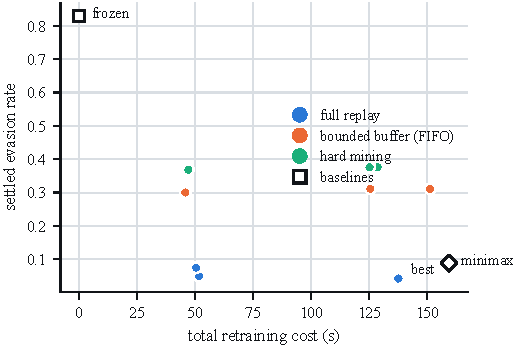
\includegraphics[width=\columnwidth]{fig5_frontier}
\caption{Robustness versus retraining cost. Lower is more robust, left is
cheaper. Hollow markers are the frozen and minimax baselines.}
\label{fig:frontier}
\end{figure}

\section{Discussion}

The practical reading is blunt. A vendor deciding how to spend an adversarial
retraining budget should spend it on \emph{retaining adversarial samples}, not
on retraining more frequently: within this design, tripling retraining
frequency is statistically indistinguishable from not doing so, while raising
the replay capacity from $200$ to $800$ samples moves settled evasion from
$0.31$ to $0.04$.

The capacity result also simplifies the design problem rather than complicating
it. Because performance saturates---$800$ retained samples already matches
unbounded replay---the practical question is not \emph{which} adversarial
samples to keep but simply \emph{whether the buffer is above threshold}. Above
it, eviction policy is a free choice; below it, the intuitive
optimisation---keep only the hardest examples, since they are the most
informative---is actively harmful. We would expect the threshold itself to
scale with the diversity of the attack rather than being a universal constant,
and locating it for a given deployment is a cheap, one-dimensional sweep.

Two methodological points generalise beyond this dataset. First, a
co-evolution benchmark is only measuring the defence if the attacker's
reachable set is not something the defender can memorise in one round; a fixed
attack strategy produces a knockout that looks like a defensive success.
Second, the encoding of \emph{which features the adversary may modify} is not a
detail of the threat model but the dominant determinant of the result, and
should be reported and justified as prominently as the model architecture.

\section{Limitations}

The attack is \emph{feature-space}: the adversary perturbs EMBER vectors, not
PE files, so the reported rates are not measured against binaries that were
verified to still execute. Bridging to the problem space requires a malware
corpus under institutional and legal control and is future work.

The main study uses a stochastic mimicry attacker because the RL agents we
implemented apply substantially weaker pressure. We therefore claim the policy
ordering holds \emph{for an attacker strong enough to create meaningful
pressure}; establishing that it also holds under a strong \emph{learned}
attacker requires an RL agent competitive with mimicry, which our calibration
suggests is an open problem rather than a matter of tuning.

Results are on one corpus, one defender family, an $8$-round horizon, and an
$8000$-sample subsample. The cadence null is best read as ``no detectable
effect at this power'' rather than a demonstrated equivalence.

\section{Conclusion}

We ran the controlled comparison the iterated-malware-detection literature has
been missing: one harness, one attacker, one metric set, and the retraining
policy as the independent variable. What the defender retrains on dominates how
often it retrains so completely that cadence is not statistically detectable,
the effect is driven by replay capacity rather than by clever example
selection, and the most intuitive selection heuristic is the worst performer.
A minimax-alternation baseline is dominated by simply retraining every round.
We release the harness and all run artifacts so that the comparison can be
extended to new policies, attackers, and corpora.

\section*{Reproducibility}

Harness, configurations, analysis scripts, and every result file are released.
All figures are regenerated from the committed artifacts by a single script;
no reported number is hand-entered. The calibration results of
Section~\ref{sec:calibration} are documented separately so that the
constraints they impose are reusable.

\begin{thebibliography}{1}
\bibitem{anderson2018}
H.~S. Anderson, A.~Kharkar, B.~Filar, D.~Evans, and P.~Roth, ``Learning to
evade static PE machine learning malware models via reinforcement learning,''
\emph{arXiv:1801.08917}, 2018.

\bibitem{anderson2018ember}
H.~S. Anderson and P.~Roth, ``EMBER: An open dataset for training static PE
malware machine learning models,'' \emph{arXiv:1804.04637}, 2018.

\bibitem{quertier2022}
T.~Quertier, B.~Marais, S.~Morucci, and B.~Fournel, ``MERLIN --- malware
evasion with reinforcement learning,'' \emph{arXiv:2203.12980}, 2022.

\bibitem{ebrahimi2022}
M.~R. Ebrahimi, W.~Li, Y.~Chai, J.~Pacheco, and H.~Chen, ``An adversarial
reinforcement learning framework for robust machine learning-based malware
detection,'' in \emph{Proc. IEEE Int. Conf. Data Mining Workshops (ICDMW)},
2022, pp. 567--576.

\bibitem{bilevel2026}
``Adversarial co-evolution of malware and detection models: A bilevel
optimization perspective,'' \emph{arXiv:2604.22569}, 2026.

\bibitem{raid_hardening}
``How to train your antivirus: RL-based hardening through the problem space,''
in \emph{Proc. Int. Symp. Research in Attacks, Intrusions and Defenses (RAID)}.

\bibitem{drmd2026}
``DRMD: Deep reinforcement learning for malware detection under concept
drift,'' \emph{arXiv:2508.18839}, 2026.
\end{thebibliography}

\balance
\end{document}
